% CREATED BY DAVID FRISK, 2016
\chapter{Background}

\section{IoT}
As mentioned in Section~\ref{sec:intro_iot} IoT is the concept of connecting all things to create a “smart world”. With the release of IPv6 the development of IoT was given the opportunity to expand. Because, of the now huge address space that was made available.  According to \citet{leibson_2008}: “So we could assign an IPV6 address to EVERY ATOM ON THE SURFACE OF THE EARTH, and still have enough addresses left to do another 100+ earths.  It isn’t remotely likely that we’ll run out of IPV6 addresses at any time in the future”.

There does therefore not exist any limitations for the possibility to connect a thing to the Internet. The challenge can instead be found in the complexity of developing an IoT applications and the following security problems because of this complexity \citep{sivieri2012wsn}.

The scenario for an IoT application is often that it has concurrent event sources, unreliable communication between things and that it needs to be able to work reliable in the existence of these problems. According to \citet{armstrong2010erlang} functional programming languages are good for writing highly concurrent application with many process’ that at the same time are fault-tolerant in a reliable manner. Functional languages could because of this be a candidate for writing IoT applications \citep{haenisch2016case}. 

Functional languages can also easily describe the functionality of data processing. The data in an application is usually only processed once and this is when it is created. At this time the data is often evaluated in some manner, e.g. for detecting errors. The processing activities that do these activities in an application can therefore be seen as a set of mathematical functions operating on a stream of values. Where each function creates a new stream of values that can be used in another function to process the data \citep{haenisch2016case}. 

The security problems that can be found in IoT applications that a functional language can help prevent is done by the fact that the code size is more concise in a functional language than in an imperative language in a case like the case described above. There does not exist any formal proof for the assumption that a functional language produces more concise code but there are some anecdotal cases, for example \citet{carmack2013} that show that it could be that functional languages reduces the code size.

\citet{ray2014large} show that there is a clear correlation between code size and error rate. Therefore, using a functional language that reduces the code size of an application is one way to reduce the security risks by minimizing the amount of errors. This becomes relevant because it is not always easy to update an IoT application.

One final advantage of using a functional language over an imperative language is that it reduces the side effects. The reduction of side effects by using “pure” functions in a functional language in an IoT application means that there are fewer bugs and from this it follows that the security of the application increases \citep{haenisch2016case}.

\section{WSN}
WSNs are the next evolution of sensor and actuator networks that has been around for decades. Its task is to solve what is commonly known as the last meter problem, where the installation process is expensive and complicated. Additionally, connectors and cables can with time become loose, lost, misconnected or the hardware can even break \citep{yang2014internet}. 

Because of the length of the name “wireless sensor and actuator networks” the name “wireless sensor networks” have been adopted by most people when wireless sensor and actuator networks are talked about.  A WSN is a set of sensor nodes, where a sensor is a low-cost package that enables the integration of wireless communications, sensors and signal processing. A challenge in a network of sensors in a WSN is that a sensor is often required to have low energy consumption and specific coverage requirements and that it is bound by latency \citep{essameldindevice, yang2014internet}.

In the past the expansion of WSNs has been limited because of the lack of standardization of technologies in the case of communication in the network and at the application level. Communication with higher data throughout has been the main focus in the industry and this has resulted in that the short-range wireless connectivity techniques has been left behind \citep{gutierrez2004low}.

There are many areas where WSNs can be used but an important feature that is required of a WSN is that that it is easy to connect sensors to the network, because a network can consist of a large number of sensors \citep{gutierrez2004low}. In the following list found in \citet{yang2014internet} an example of application areas of a WSN is shown:

\begin{itemize}
   \item Continues sensing for environmental and condition monitoring.
   \item Event detection for disaster response.
   \item Location sensing for mobile target tracking and localization.
   \item Local control for home automation, industrial automation etc.
\end{itemize}

In all the application areas in the list above there are some high-level issues for designing and implementing a WSN, power consumption, range, availability of frequency bands, network topology and self-organization, that needs to be considered when designing a WSN \citep{gutierrez2004low}.

The power consumption of some applications is sometimes required to be very small. Sometimes, they are using batteries as power source with completely untethered RF transceivers. The idea of a WSN is as mentioned that is should be easy to install and have a low-cost operation. If the application requires that batteries often needs to be replace, it goes against the idea of a WSN. To solve this problem, the common solution is instead to use power cycling. If the duty cycle is of less than 0.2\% an AAA battery with the capacity of 750mAh can power a normal short-range radio transceiver, with a active current of 10mA, for at least five years. 

The range issue between a transmitter and receiver arises because of implementation costs and governmental regulation that do so the RF power output in a wireless system operating in unlicensed bands normally ranges between 0 dBm to 20 dBm. To side-step this issue in a WSN a multihop network protocols are used with a suitable routing algorithm.

The issue wit the availability of frequency bands comes from that the RF spectrum is often regulated by governments with a set of rules that needs to follow and that it is a scarce resource. The most commonly used bands in WSNs is the following bands:

\begin{itemize}
   \item 868.0-868.6 MHz: Available in most European countries.
   \item 902-928 MHz: Available in North America.
   \item 2.40-2.48 GHz: Available in most countries worldwide.
   \item 5.7-5.89 GHz: Available in most countries worldwide.
\end{itemize}

Another, issue that arises because of the limited band space is the challenge of incompatible technologies sharing the same band. This leads to that different technologies will compete to gain and maintain access to the network. From this follows that there arise several performance problems.

The requirements of the network topologies in a WSN is that it solves the problem with limited range and that the network needs to be low maintenance. The limited range problem is solved by using multihop network topologies that forms a communications mesh. To solve the low maintenance requirement of the network, the network should be designed so each sensor in the network can be developed with a low duty cycle operation.

The last high-level issue for designing and implementing a WSN is that the network needs to be self-organizing. Each sensor in the network should be able to start participating in the network without any configuration from a second party and that a suitable routing protocol is used in the network to determine an appropriate message path from a source to a destination.


\section{Erlang}
Ericsson started to develop of Erlang in 1987 with the aim of improving the development of telephony applications. The first version of Erlang was implemented in Prolog but this interpreter was far too slow. So, in 1992 the development of the BEAM virtual machine (VM) was started and it compiles Erlang to C using a mix of natively compiled code and threaded code to strike a balance between performance and disk space \citep{armstrong1997development}.

The Erlang language was developed to support distribution, concurrency and fault-tolerance and it is a general-purpose, concurrent, functional programming language. It also has a garbage-collected runtime system \citep{armstrong1996erlang}. 

To avoid side effects the Erlang language supports single assignment variables and immutable data and as other functional languages recursive functions is used instead of loop constructs. The Erlang language is also a declarative language. A declarative language is a language that instead of saying how something shall be computed, a language that describes what shall be computed. An example of declarativity in the language is the use of pattern matching to distinguish between message types. 

 One characteristic that distinguishes the pattern matching of Erlang, even though it is a high-level language is that it is possible to pattern match on binary data. Because the language was designed for embedded system this was included and it gives the possibility to implement high-level descriptive functions for packet manipulations or design of low-level communication protocols \citep{sivieri2012erlang}. An example of how pattern matching can be used can be seen in Listing~\ref{erlang_background_code1}.

\begin{minipage}{\linewidth}
\lstinputlisting[language=Erlang, label={erlang_background_code1},caption={Code example that show pattern matching and message passing.},captionpos=b,xleftmargin=2em,frame=single,framexleftmargin=1.5em,numbers=left,numberstyle=\small]{figure/erlang_background_code1.erl}
\end{minipage}

Another characteristic feature of Erlang is that an Erlang process is light weight. This means that the effort that is needed to create and destroy a process requires very little computational effort. In the Erlang language there is primitives that makes it easy to spawn new processes and because a process does not correspond directly with system processes or threads but are handled by the VM, it is possible to run many thousands of processes at the same time without degrading the performance of the system \citep{armstrong2003concurrency}. 

Each process in Erlang have a share nothing semantics. By not having any shared data it is easy to create a distributed program by assigning a parallel process to another machine and the code can be highly effective because no semaphores of mutexs are needed \citep{armstrong2003concurrency}.

The only way for a process to communicate with another process in Erlang is to pass messages. An example of message passing is shown in Listing~\ref{erlang_background_code1}. Each process has a mailbox that receive messages when a process sends a message to the id of a specific process. These messages are the only way to achieve synchronization between processes in an Erlang program \citep{armstrong2003concurrency}.

With the previous mention characteristics of Erlang, it is easy to make a system fault-tolerant by using a mechanism that is called process linking. A process can spawn another process and by linking to the spawned process it can receive exit messages. If exit message is an error message the process that observe a spawned process can perform error recovery \citep{armstrong2003concurrency}. This error recovery procedure is often called a supervisor and by using the supervisor behaviour from the Open Telecom Platform (OTP) library trees of processes can be created. Where every observed process can be defined with a specific restart behaviour to handle error recovery \citep{armstrong2003concurrency, sivieri2012erlang}. 

Erlang also supports hot code swapping. This allows Erlang models to be updated on the fly without the need to stop running the system and to make sure that the old code terminates gracefully \citep{sivieri2012erlang}.

One last thing to mention about Erlang is that it provides some different alternatives for running C code. The alternatives are ports, port drivers, C nodes and Native Implemented Functions (NIFs). The difference between these methods are in how they are loaded. For example, NIFS are dynamically linked into the emulator process and port drivers are a shared library and these methods to load the C code would case the emulator to crash if the C code terminates. A representation of the loading differences between a port and a port drivers can be seen in Figure~\ref{fig:erlang_run_ccode} \citep{ericsson_ab_2019}. 

\begin{figure}[H]
\centering
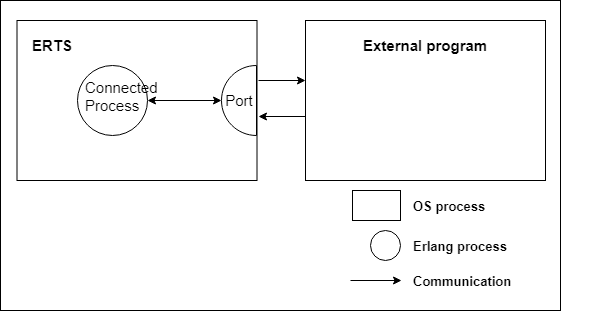
\includegraphics[scale=0.5]{figure/erlang_port.png}
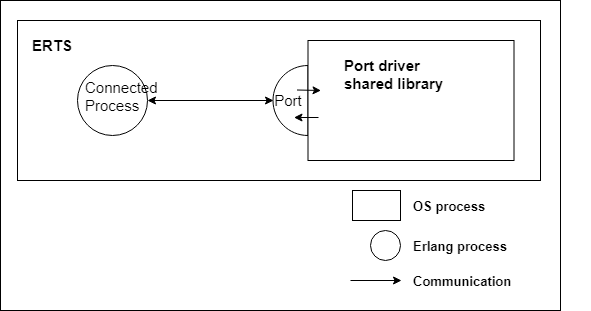
\includegraphics[scale=0.5]{figure/erlang_port_driver.png}
\caption{Port and port driver communication.}
\label{fig:erlang_run_ccode}
\end{figure}

\section{IEEE 802.15.4}
The communication standard that is usually used within the Internet is the TCP/IP architecture. The architecture consists of five functional layers, the physical, data-link, network, transport and application layers. When data is passed between these layers extra framing and control data is added to the main data. This added data requires extra processing power and memory capacity and even more memory and processing power are consumed because of buffering of packets between the different layers \citep{BELLO201752}.

One additional limitation of the TCP/IP protocol is that it is not designed to manage device-to-device communication. It has no support for the high level of scalability, high amount of traffic and mobility that can be found in WSNs \citep{BELLO201752}. One of the most commonly used communication standards to solve this problem is IEEE 802.15.4 standard \citep{yang2014internet}.

The IEEE 802.15.4 standard was first published in 2003 as a low-rate Wireless Personal Area Network and it was developed to provide wireless connectivity in a low-complex, low-cost and low-power manner. 

\subsection{Components}
There are two types of devices that an IEEE 802.15.4 network consists of, a full-function device (FFD) and a reduced-function device (RFD).  The PAN coordinator serves as the central device in a network and is responsible for starting and managing the network. An FFD device can freely communicate with all devices within range and the coordinator is an FFD device that has been assigned as the PAN coordinator. The RFD device is a restricted device and can only communicate with its parent FFD device \citep{yang2014internet}.

\subsection{Network topologies}
The IEEE 802.15.4 standard defines to network topologies, the star topology and peer-to-peer topology. Both topologies are shown in Figure~\ref{fig:topologies} and both topologies needs to have a personal area network (PAN) coordinator. A PAN coordinator is an FFD device that has been assigned as the coordinator of the network \citep{kohvakka2006performance}.

\begin{figure}[H]
\centering
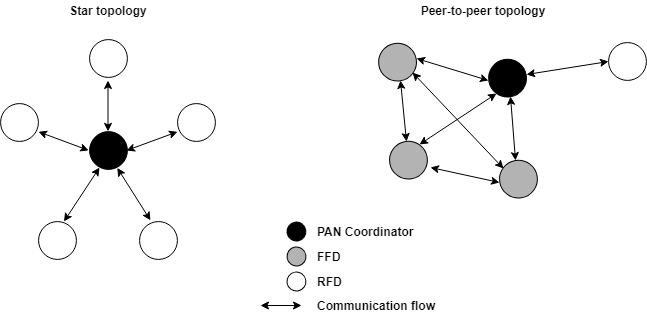
\includegraphics[scale=0.6]{figure/topologies.png}
\caption{IEEE 802.15.4 topologies}
\label{fig:topologies}
\end{figure}

The difference between a star network and a peer-to-peer network is that in a star network the PAN coordinator is the master node. All slave nodes of the network can only communicate with this master node \cite{kohvakka2006performance}. This is achieved when an FFD device is initiated as a PAN coordinator and a unique PAN identifier in the current radio range is selected. When other devices associate with the network, they get the same PAN identifier and can only communicate with the PAN coordinator of the network with the same PAN identifier \citep{lan2003part}.

In a peer-to-peer network all devices are allowed to communicate with any other device in the network. This is suitable for networks where self-organizing, self-healing and large coverage by allowing multiple hops to route messages is an advantage. A disadvantage that follows from this is that the network latency increases due to the message relaying \citep{kohvakka2006performance}.

\subsection{Architecture}
The standard is for the two first layers in the network stack, the Physical (PHY) and Medium Access Control (MAC) layers. Where the PHY layer contains the radio frequency transceiver and the low-level mechanisms that is needed to operate the transceiver.  

\vspace{5mm}
\textbf{PHY layer}

The PHY layer is divided in two, where one part operates in the frequency range 868-868.6 MHz in Europe or 902-928 MHz in America and the other part at 2.4 GHz worldview \citep{lan2003part, zigbee2007spec}. The second part has the most potential for WSNs, because the high data rate leads to a reduced frame transmission time and a reduced energy per transmitted and received bit \citep{kohvakka2006performance}.

\citet{7460875} defines the features of the PHY layer as following features: 

\begin{itemize}
   \item Activation and deactivation of the radio transceiver.
   \item Energy detection within the current channel.
   \item Link quality indicator for received packets
   \item Clear channel assessment for carrier sense multiple access with collision avoidance (CSMA-CA). 
   \item Channel frequency selection.
   \item Data transmission and reception.
   \item Precision ranging for ultra-wide band PHYs.
\end{itemize}

\vspace{5mm}
\textbf{MAC layer}

Two services are provided by the MAC layer. The first one is the MAC data service and it provides functionalities that makes it possible for transmission and reception of MAC protocol data units across the PHY data service. The second service is the MAC management service. It provides an interface to the MAC sublayer management entity (MLME) service access point \citep{7460875}.

\citet{7460875} defines the features of the MAC layer as following features: 

\begin{itemize}
   \item Beacon management.
   \item Channel access.
   \item GTS management.
   \item Frame validation. 
   \item Acknowledged frame delivery.
   \item Association, and disassociation.
   \item Hooks for implementing application-appropriate security mechanisms.
\end{itemize}



\section{ZigBee}
On top of the IEEE 802.15.4 standard are built the most commonly used protocols in WSN applications, 6LoWPAN and ZigBee. They are currently independent of each other, where 6LoWPAN gives sensors the possibility to be accessed from the Internet as opposed to ZigBee, which cannot do this because it lacks native IP stack processing. The protocol stack for 6LoWPAN and ZigBee can be seen in Figure~\ref{fig:protocolstacks}.

\begin{figure}[H]
\centering
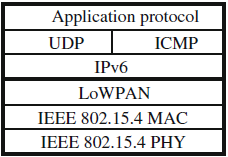
\includegraphics[scale=0.4]{figure/6LoWPANstack.png}
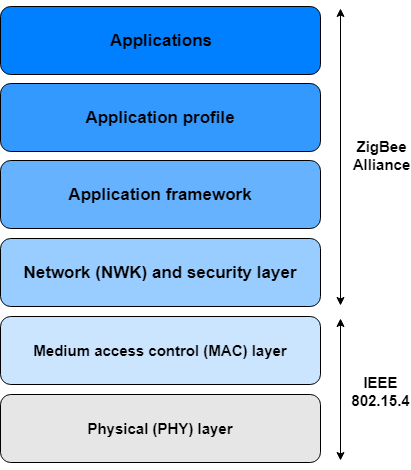
\includegraphics[scale=0.4]{figure/ZigBeestack.png}
\caption{6LoWPAN stack and ZigBee stack on top of the IEEE 802.15.4 stack}
\label{fig:protocolstacks}
\end{figure}

In Table~\ref{table:zigbee_comparison} a comparison of the characteristics between ZigBee, Bluetooth and WiFi are presented.

\begin{table}[H]
\centering
\resizebox{\columnwidth}{!}{%
\begin{tabulary}{\textwidth}{LLLL}
\toprule
    &  ZigBee (IEEE 802.15.4) & Bluetooth (IEEE 802.15.1) & WiFi (IEEE 802.11) \\ 
\midrule
Application             & Control and monitoring         & Cable replacement &  Wireless LAN\\
Frequency bands         &  2.4 GHz, 868 and 915 MHz      & 2.4 GHz           &  2.4 GHz\\
Battery life (days)     &  100–700                       & 1–7               &  0.1–5\\
Node per network        &  65,000                        & 7                 &  30\\
Bandwidth               &  20–250 kbps                   & 1 Mbps            &  2–100 Mbps\\
Range (m)               &  1–300                         & 1–10              &  1–100\\
Topology                & Star, tree, cluster tree, mesh & Tree              &  Tree\\
Standby current (Amps)  & $3*10^{-6}$                    & $200*10^{-6}$     &  $20*10^{-3}$\\
Memory (KB)             & 32–60                          & 100               &  100\\ 
\bottomrule
\end{tabulary}%
}
\caption{ZigBee, Bluetooth, and WiFi comparison \citep{yang2014internet, zigbee_alliance_2019}}
\label{table:zigbee_comparison}
\end{table}

\subsection{Architecture}\label{sec:architecture}
The architecture of ZigBee can be seen as a set of blocks, that is usually called layers. Each layer is tasked with preforming a specific service for the layer above and the layer below another layer have no knowledge about the layer above it. Between each layer there is two Service Access Points (SAPs) that isolates a layer. One of these SAPs provides a data transmission service and the other provides a management entity service that control all other services in the attached layer by exposing an interface for the layer above \citep{gislason2008zigbee, zigbee2007spec}. An image that represents the architecture of the ZigBee stack can be found in Figure~\ref{fig:zigBeeArch}.

\begin{figure}[ht]
\centering
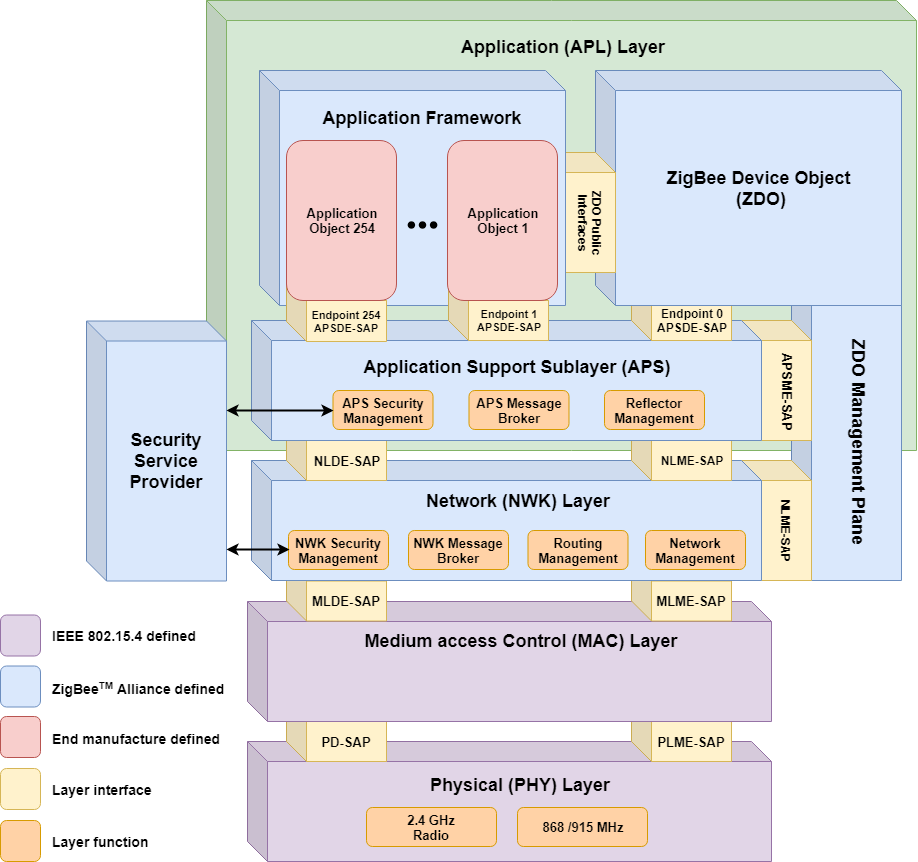
\includegraphics[scale=0.46]{figure/ZigBeeStackArchitecture.png}
\caption{Image of the ZigBee stack architecture based on ideas from \citet{gislason2008zigbee, yang2014internet, zigbee2007spec}.}
\label{fig:zigBeeArch}
\end{figure}

\vspace{5mm}
\textbf{Application layer (APL)}

The APL consist of the Application Support Sublayer (APS), ZigBee Device Object (ZDO) and manufacture defined application objects \citep{zigbee2007spec}.

The APS is the layer above the Network (NWK) Layer and provides the NWK layer with an interface to the APL.  The task that the APS has is to filter out packets where endpoints does not exist, manage transmission retries with end-to-end acknowledgment, maintaining the local binding table which handles the connection of an endpoint on the current node with one or more endpoints on other nodes, maintaining the local groups table which makes it possible to send group-addressed frames to endpoints associated with the same group and maintaining the local address map which handles the association between a 64-bit MAC address with a ZigBee 16-bit network address \citep{gislason2008zigbee, zigbee2007spec}.

The ZDO is an application that on every ZigBee device runs on endpoint 0 and includes the ZigBee Device Profile. This is a specialized application profile that on a network is responsible for discovering, configuring and maintaining ZigBee devices and services.  The ZDO applications also directly interacts with the NWK layer, by controlling when to create a network or join a network and when to leave a network \citep{gislason2008zigbee}.

Manufactured defined application objects are resides in the Application Framework (AF). The AF also contains the ZigBee Cluster library and the task of this library is to provide a framework for running applications where each application has a unique endpoint \citep{gislason2008zigbee}.

\vspace{5mm}
\textbf{Network (NWK) layer}

The task of the NWK layer is to connect the above layers with the MAC sub-layer. To connect with the APL, the NWK layer as all other layers also provides two SAPs as described in Section~\ref{sec:architecture}. The data service and management service that the SAPs corresponds to are responsible for \citep{farahani2011zigbee, zigbee2007spec}:

\begin{itemize}
   \item Transporting protocol data units to intended recipients.
   \item Provide security that ensure both authenticity and confidentiality of a transmission.
   \item Self-configuration of the stack for either starting a network as a ZigBee coordinator or joining a network.
   \item Create a new network. 
   \item The ability to for a device to join, rejoin and leave a network. This also include the ability for a ZigBee coordinator or router to request that another device leave the network.
   \item Address assignment of a device by a ZigBee coordinator or router.
   \item Discovering, recording and reporting information about devices directly neighbourly to the current device.
  \item Discovering and recording paths for sending messages.
  \item Controlling when the recipient device is active and for how long and by this enabling MAC sub-layer synchronisation or direct reception.
  \item The ability to use routing mechanisms such as unicast, broadcast, multicast and many to one to exchange data in the network efficiently.
\end{itemize}

\vspace{5mm}
\textbf{Security service provider}

The security service provider is responsible for services that provides encryption of data confidentiality, device and data authentication and replat protection. These security measures are optional, and it is up to the developer to chose if they should be used \citep{farahani2011zigbee}.

\subsection{Network topology}
The network topologies available in ZigBee are based on the star and peer-to-peer topologies specified in IEEE 802.15.4. Based on these topologies from IEEE 802.15.4 the NWK layer of the ZigBee stack supports star, tree and mesh topologies \citep{farahani2011zigbee}.

The star topology is the simplest topology to form. When an FFD device that is programmed to be a PAN coordinator starts, it establishes a network. Every device that wants to join the network must join the network through the PAN coordinator. Because of this the star topology is not suitable for application that requires a bigger area than the radio range of the PAN coordinator \citep{yang2014internet}.

\begin{figure}[H]
\centering
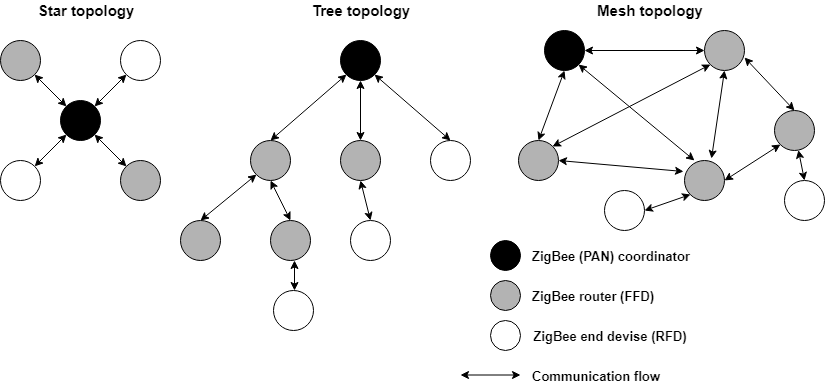
\includegraphics[scale=0.5]{figure/zigbeetopologies.png}
\caption{ZigBee network topologies}
\label{fig:zigbeetopologies}
\end{figure}

The peer-to-peer topology gives the possibility for different shaped networks. In a tree topology (see Figure~\ref{fig:zigbeetopologies}) a PAN coordinator creates the network, FFDs forms the branches of the tree and RFDs are the leaves. The difference between a tree topology and a mesh topology (see Figure~\ref{fig:zigbeetopologies}) is that in the tree topology there exist restrictions on the communication between FFDs. In a mesh topology every FFD can communicate with all other FFDs in radio range. Figure~\ref{fig:barrier_topology} shows the advantage one of the peer-to-peer topologies have in extending the range of the network and even circumvent barriers \citep{farahani2011zigbee}.

\begin{figure}[ht]
\centering
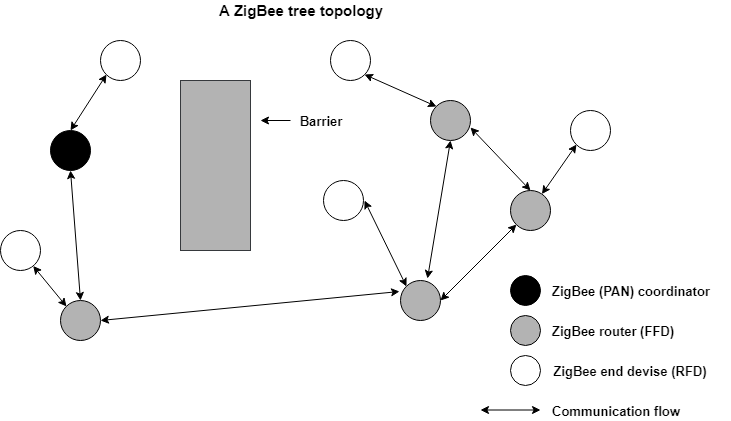
\includegraphics[scale=0.5]{figure/barrier_topology.png}
\caption{A ZigBee network topology with a barrier.}
\label{fig:barrier_topology}
\end{figure}
